% !TeX spellcheck = en_US
\documentclass[compsoc,onecolumn,11pt,a4paper,final]{IEEEtran}

%%% Packages
\usepackage[utf8]{inputenc} 			% for umlautes
%\usepackage[ngerman]{babel} 			% for German
\usepackage[T1]{fontenc} 				% adjust font encoding in output
\usepackage{amsmath} 					% enable mathematical symbols
\usepackage[cmintegrals]{newtxmath}		% ieee style for integrals
\usepackage{xargs}                      % use more than one optional parameter in a new commands
\usepackage[pdftex,dvipsnames]{xcolor}  % coloured text etc.
\usepackage{graphicx}
\usepackage{caption}
\usepackage{float}						% forcing figure here (H option)
\usepackage{ifdraft}					% \ifdraft{do in draft}{do in final}
\usepackage{hyperref}					% PDF-Links and Bookmarks
\usepackage{bookmark}
\usepackage{mathtools}
\usepackage{soul}						% \st for strike through
\usepackage{lipsum}						% dummy text

%%% Tikz
\usepackage{pgf,tikz}
\usepackage{mathrsfs}
\usetikzlibrary{arrows}

%%% Colors
\definecolor{red}{rgb}{1,0,0}
\definecolor{green}{rgb}{0,1,0}
\definecolor{blue}{rgb}{0,0,1}

%%% TODO nots
\usepackage[colorinlistoftodos,prependcaption,textsize=tiny]{todonotes}
\newcommandx{\unsure}[2][1=]{\todo[linecolor=red,backgroundcolor=red!25,bordercolor=red,#1]{#2}}
\newcommandx{\change}[2][1=]{\todo[linecolor=blue,backgroundcolor=blue!25,bordercolor=blue,#1]{#2}}
\newcommandx{\info}[2][1=]{\todo[linecolor=OliveGreen,backgroundcolor=OliveGreen!25,bordercolor=OliveGreen,#1]{#2}}
\newcommandx{\improvement}[2][1=]{\todo[linecolor=Plum,backgroundcolor=Plum!25,bordercolor=Plum,#1]{#2}}
\newcommandx{\thiswillnotshow}[2][1=]{\todo[disable,#1]{#2}}

%%% Title and author
\title{CSP and SAT Encoding}
\author{ 
	\IEEEauthorblockN{Mazen Bouchur}\\
	\IEEEauthorblockA{TU Clausthal, Germany}
}

\begin{document}
\maketitle
	
\begin{abstract}\label{abstract}
This paper gives a brief overview over different encodings between the constraint satisfaction problem (CSP) and the Boolean satisfiability problem (SAT). 
Each encoding is analyzed and evaluated based on various aspects and characteristics such as performance and complexity. 
Most importantly each encoding is being compared performance-wise to the unencoded counterpart with respect to the standard algorithm of each problem (DPLL in case of SAT and arc consistency based algorithm in case of CSP).
We try to summarize multiple papers discussing several encodings and highlight the remarkable properties of each them, specially the SAT-based constraint solver "sugar" and its underlying order encoding.
\end{abstract}

% !TeX spellcheck = en_US
\section{Introduction}\label{sec:intro}
\subsection{SAT}
%%% Importance
Ever since it was formulated and the Boolean satisfaction problem (SAT) is gaining an increasing interest in the field of computer science. It has a wide range of applications in various areas, ranging from hardware design to artificial intelligence (AI) and verification. SAT can be used to express many AI tasks and mathematical problems as a constraint satisfaction problems. Other theoretical applications also include automated theorem proving and model checking.

SAT can be defined as the problem of finding an assignment of the propositional variables of given Boolean formula, such that the whole formula evaluates to True (satisfied).
%%%% Other
SAT is one of the first problems that was proven to be NP-complete, which makes it gain increased importance.
Being simple in its nature and construction has allowed intensive studying and optimization. Therefore, the efforts to converting problems into SAT instances to benefit from its advantages should come as no surprise.
Throughout this paper it is assumed that the SAT problem is expressed in clausal CNF form to facilitate a common basis. % TODO

\subsection{CSP}
%(On the other hand)
Many famous problems such as the n-queens’ problem, map coloring and Sudoku can be easily expressed as an instance of the constraint satisfaction problem (CSP). Each CSP consists of three sets: 
\begin{enumerate}
	\item Set of variables.
	\item Set of domains for each variable (usually a finite domain is chosen for all the variables).
	\item Set of relations that define the constraints over a subset of the variables’ set.
\end{enumerate}

\subsubsection{CSP Types}
Based on the number of the participated variables, a constraint can be classified as unary, binary or n-ary constraint. The entire CSP can be described as binary or non-binary depending on the constraints’ classification. To be consistent and for facilitate theoretical analysis only unary and binary CSP are considered in this paper.Any n-ary can be expanded and expressed in terms of binary constraints.

%Studying the relationships and connections between those problems:
% TODO 	Exploit the fact that SAT is better studied and simpler in CSP solving\\

% !TeX spellcheck = en_US
\section{Preliminaries}\label{sec:prelim}
In this section, the algorithms used for solving each problem and the basis criteria for the theoretical comparison between them will be formally introduced. 

\subsection{The Davis-Putnam-Logemann-Loveland algorithm (DPLL)}
One technique to solve the satisfiability problem is the Davis-Putnam-Logemann-Loveland (DPLL) algorithm, which is a refinement of the original resolution-based Davis-Putnam (DP) algorithm. DPLL is based on four rules:
\begin{enumerate}
	\item Tautology elimination
	\item One Literal (Unit clause)
	\item Pure Literal
	\item Branching or splitting
\end{enumerate}
For our purposes, just the one literal and the branching rules will be considered as they are sufficient for the completeness and soundness of the algorithm, and none of the other rules affect the efficiency.

%%% Important rules (2+4) quick explanation
\textit{One Literal:} This rule eliminates unit clauses (any clause contains a single unassigned literal) by assigning the only possible value to make this literal true. Thus, no choice is necessary. By applying this rule, a large part of the entire search space can be pruned, leading to a more efficient SAT instance that is equivalent to the original problem.

\textit{Branching:} When no other rule is applicable, branching is used to assign a truth value to a variable. This assignment is non-deterministic and depending on the used branching-heuristics a variable is chosen. 

An unsatisfiable SAT problem will lead to apply branching and unit propagation to all branches until no variable is left. For this reason, it is usually harder to detect unsatisfiability, since all branches must be traversed.

\subsection{Arc consistency and the forward checking algorithm (FC)}
A standard approach to solve the constraint satisfaction problems is maintaining arc consistency (MAC) or forward checking (FC). Both algorithms are built around the idea of enforcing some level of arc consistency (AC) at each step and branch when needed. The main difference between FC and MAC is the fact that MAC tries to maintain AC on each node at every level while FC tries to avoid the extra work by maintain AC only between the most recently instantiated variables and those that are still not instantiated.

While FC do in general much less work at each node, it needs to branch much more to exclude all wrong paths. On the other hand, MAC usually have smaller number of branches and spends in return more time at each node. This trade-off leads to different characteristics of each algorithm, which in turn prioritize one over another according to the concrete problem.
% TODO where to cont. ....one can better than the other

\subsection{Analysis approach}
To determinate that an encoding is good enough or rather better than another (see below), we will compare solving a given problem with its standard algorithm to solving the encoded version of the same problem with its respective standard algorithm. For example: A CSP problem can be solved directly using MAC or it can be encoded as SAT problem (using order encoding for instance) and solved using DPLL. Note that the encoding process cannot take longer time than solving the problem itself. In concrete terms, the encoding procedure (which can be considered as reduction) can be done in polynomial time since both problems are NP complete.

\subsubsection{Branching for comparing}
Since both MAC/FC and DPLL are backtracking based approaches, we will use the number of visited branches as indicator for the efficiency of each algorithm and in this way compare the impact of achieving arc-consistency from FC on the CSP with unit propagation from DPLL on the SAT problem. So, one algorithm outperforms (dominates) another if and only if it visits less number of branches assuming equivalent branching heuristics.

This criterion has been chosen because it serves as a good indicator for the performance of these algorithms in real world applications. This comparison will be aided with examples and comparisons at the end of the paper.
Notice that considering this criterion, FC is always dominated by MAC which does not always reflect the real performance but gives a good clue about the efficiency of each algorithm without diving too deep into the exact implementation.

% !TeX spellcheck = en_US
\section{CSP into SAT encoding}\label{sec:csp_to_sat}
Mapping a CSP problem into a SAT instance can be done in many ways. Several methods of encoding a CSP instance as a propositional formula have been proposed. Some of the most common encodings will be introduced in this section.

% !TeX spellcheck = en_US
\subsection{Direct encoding}
As the name suggests, the direct encoding assign for each CSP variable $x$ and for each possible value from its domain $i$ a new propositional variable $x_i$ on the SAT side. The boolean variable is then True if and only if the original variable is assigned the value $i$.  To ensure consistent logical assignment for each propositional variable, we need to extend the SAT problem to include clauses that avoid inconsistent results such as assigning a CSP variable two values at the same time or no value at all (at-least-once and at-most-once clauses) \cite{petke2011order}.

\subsubsection{Example}
Consider the following instance of the map coloring problem:\\
\begin{figure}[H]
	\centering
	
\includegraphics[width=0.5\linewidth]{assets/map_coloring_unsolved}
	\captionsetup{justification=centering,margin=2cm}
	\caption{Unsolved instance of the map coloring problem}
	\label{fig:map_coloring_unsolved}
\end{figure}  
The map consists of four regions $A,B,C,D$ sharing boarder as shown in the figure \ref{fig:map_coloring_unsolved}. The purpose of this problem is to color each region of the map so that no two adjacent regions have the same color. The variables in this case are the regions themselves $\{A,B,C,D\}$ and each of them has the domain $\{r,g,b\}$ which stands for the colors red, green and blue respectively. To fully define the CSP we also need to define the constraints' set which comprise two types of constraints: 
\begin{itemize}
	\item unary constraints such as $A\neq r$ since $A$ is already adjacent to a red colored region 
	\item binary constraints such as $A\neq B, A\neq C,\dots$ i.e. no two adjacent regions share the same color
\end{itemize}
Hereafter, the unary constraints are avoided by restricting the domain of $A$ and $D$ to not include red; on the other hand, it should be noted that usually all the variables are given the same domain to simplify the problem.

Encoding this problem directly will result in the following SAT instance:
a new propositional variable is associated with each value that can be assigned to a CSP variable. So we get the variables: $\{ A_g, A_b, B_r, B_g,\\ B_b, \dots\}$. To ensure that each CSP variable will be assigned at least one color, we have to include the following at-least-once (ALO) clauses: $\{ A_g \vee A_b, B_g \vee B_r \vee B_b, \dots \}$. Similarly, we must ensure that no CSP variable is assigned multiple colors at the same time, which can be expressed as these at-most-once (AMO) clauses: $\{ A_g \oplus A_b, B_g \oplus B_r, B_g \oplus B_b, B_r \oplus B_b, \dots \} $, where $\oplus$ stands for the logical exclusive or operation $a \oplus b \equiv (a \wedge \neg b) \vee (\neg a \wedge b) \equiv (a \vee b) \wedge \neg (a \wedge b)$.
\begin{figure}[H]
	\centering
	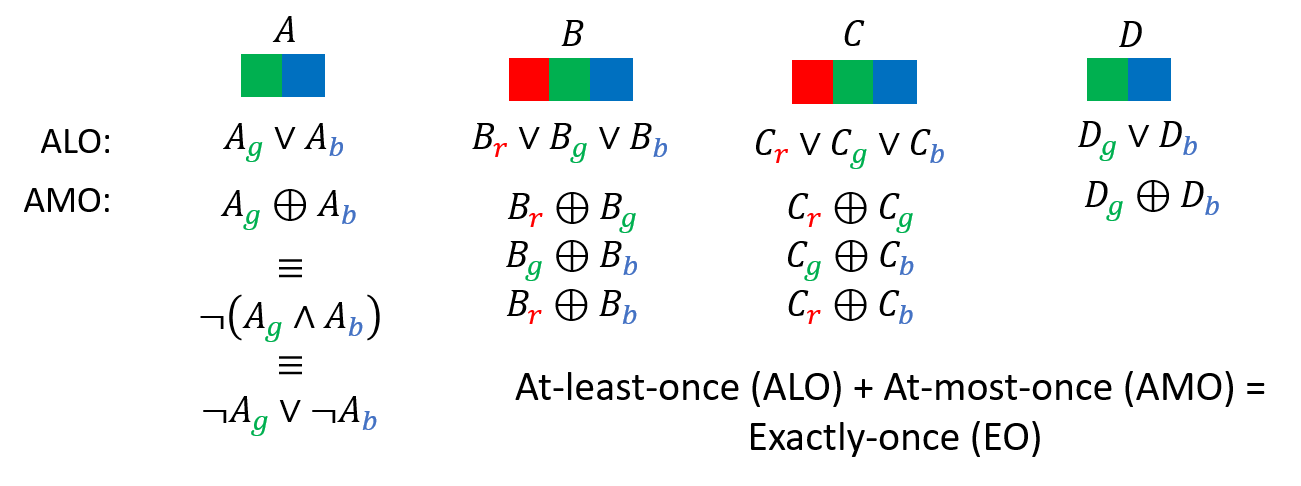
\includegraphics[width=0.75\linewidth]{assets/alo_amo}
	\captionsetup{justification=centering,margin=2cm}
	\caption{Both types of clauses in direct encoded SAT}
	\label{fig:alo_amo}
\end{figure}  
ALO and AMO clauses will enforce each CSP variable to be true only for one value from its domain, hence the name exactly-once (EO) clauses.

We still need to encode the binary constraints from CSP into some sort of clauses in SAT. This can be done easily by ensuring that no two CSP variables such as $C$ and $B$ share the same color, which can be translated into the following clauses:
$$
	\neg (C_r \wedge B_r) \quad, \neg (C_g \wedge B_g) \quad, \neg (C_b \wedge B_b)
$$
The same principle applies for the reset.
%\textcolor{red}{TODO: add a word about the similar support encoding (since both are sparse encodings)}

The direct encoding can be categorized under a general type called the sparse encoding. Notice that the direct encoding encodes conflict points (so called conflict or no-good) assignments such as $A$ and $B$ can't share the same color at the same time $\neg (A_c \wedge B_c) \equiv \neg A_c \vee \neg B_c$. It is also possible to encode the allowed (so called supports) assignments, e.g. $\neg A_c \vee B_c \vee C_c \vee D_c$. This type of clauses is the basis for the other type of sparse encoding called accordingly the support encoding \cite{petke2011order}.

\subsubsection{Proposition}
Solving the CSP problem directly with FC compared to the direct encoded SAT instance of the same CSP problem solved with DPLL will always result in similar search tree structure. i.e. FC on the original CSP problem and DPLL on the direct encoded SAT will explore the same number of branches. This proposition assumes equivalent branching heuristics for DPLL and FC.

\subsubsection{Proof idea}
Considering the generated search tree, our version of DPLL comprise only two rules: the one literal and the branching rule. This means at each node in the tree we either have to branch or the given variable must be assigned a truth value of either False or True. 

On the FC side branching is equivalent to its counterpart in DPLL. The second case in DPLL (unit propagation by the one literal rule) is also equivalent to applying forward checking by enforcing arc consistency and reducing the domain of each CSP variable to one value only.

Similarly, we can trace the whole structure of both trees and process with the same logic on each propositional variable. By induction, we can prove that each algorithm explore the same number of branches \cite{walsh2000sat}. 

\subsubsection{Example}
Compare the following search trees of FC applied to the previous map coloring problem and DPLL applied to direct encoded instance of the same previous map-coloring problem:
\begin{figure}[H]
	\centering
	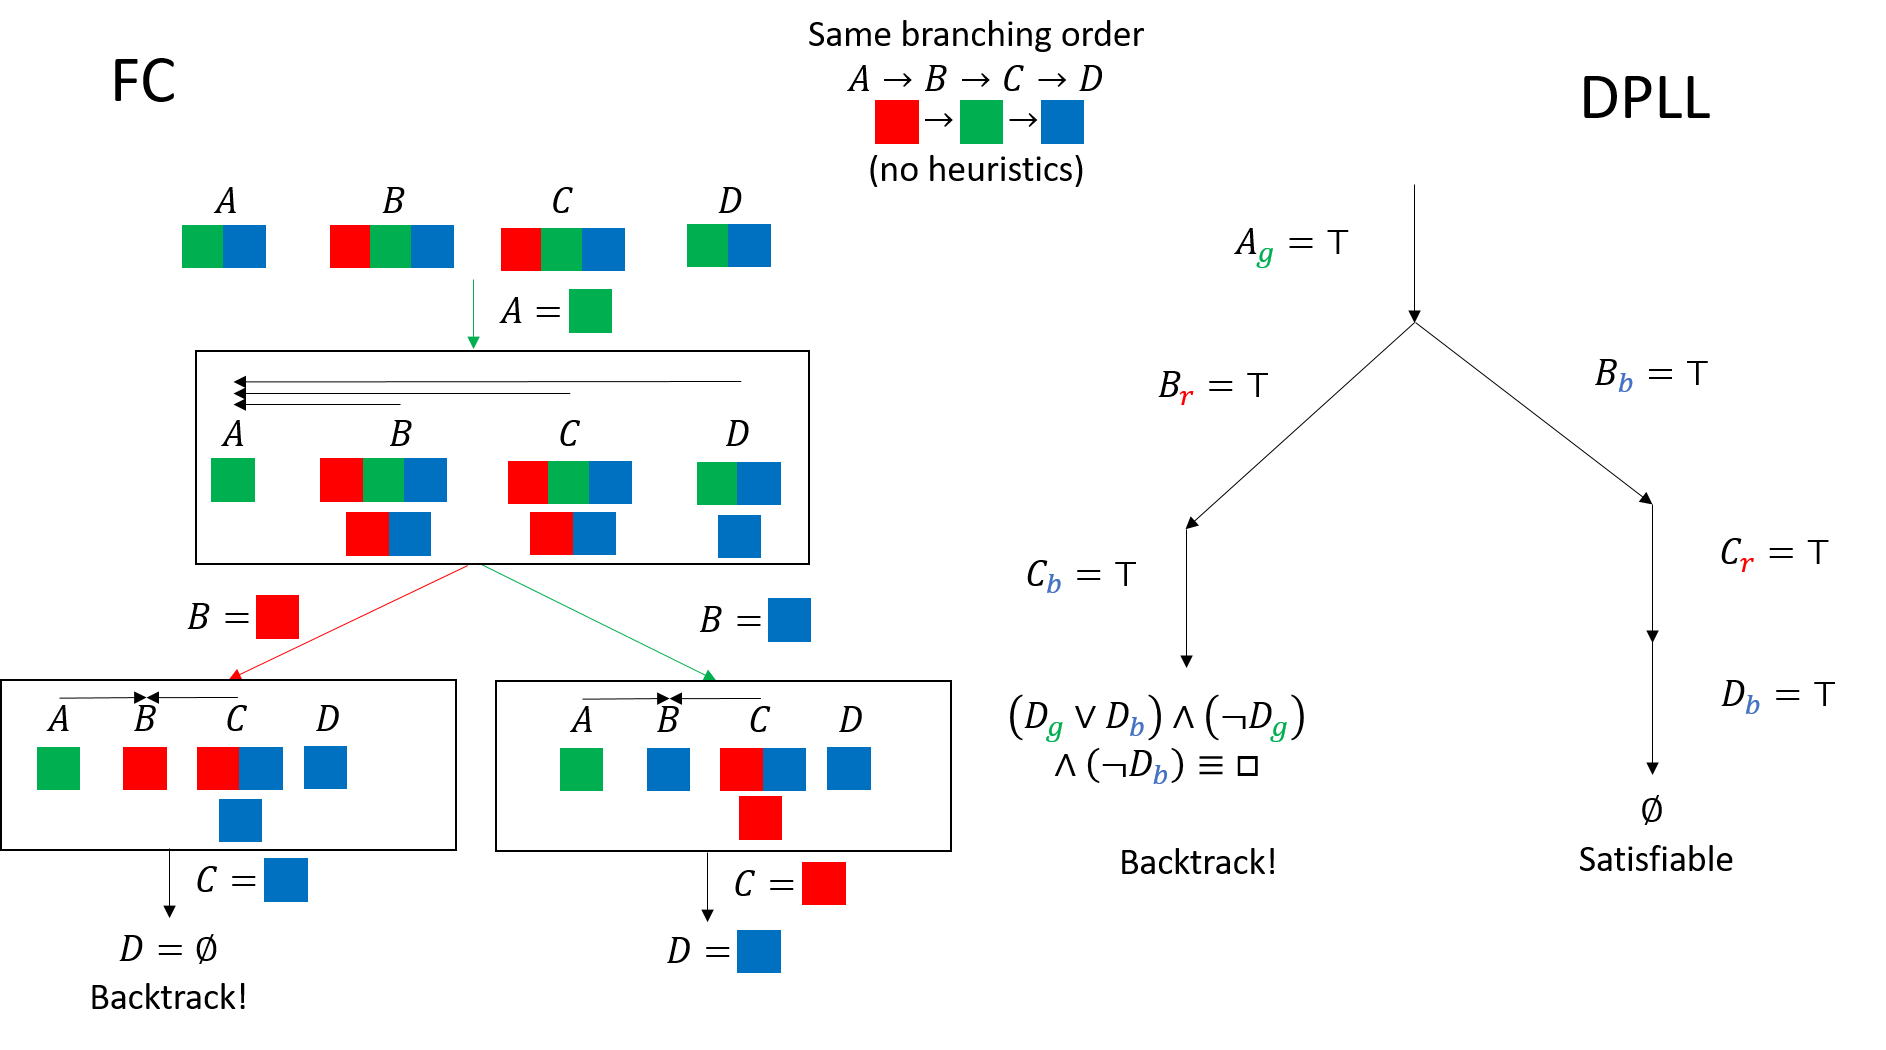
\includegraphics[width=1\linewidth]{assets/direct_fc_vs_dpll}
	\captionsetup{justification=centering,margin=2cm}
	\caption{Search trees of FC and DPLL}
	\label{fig:direct_fc_vs_dpll}
\end{figure} 
The arrows in node level on the FC side indicates enforcing arc consistency and the results are show directly underneath on the next line.





% !TeX spellcheck = en_US
\subsection{Log encoding}
This encoding utilize the fact that each propositional variable can only take one of two values.

\subsubsection{Encoding the variables}
First we encode each possible value from the domain with a distinct binary representation. Depending on the maximum number of bits needed to encoded all the domain values, an equal number of propositional variables for each CSP variable is generated. So if the size of domain was $m$ and the number of CSP variables was $n$, we need $n \lceil \log_2 m \rceil$ propositional variable on the SAT side.

Notice that encoding each value from the CSP variable's domain means that the size of this domain must be exactly equal to $2^i$, which is not always the case. So extra possible binary representations can emerge (implied in the formula by the ceiling function, i.e. if $ \lceil \log_2 m \rceil > \log_2 m $). To avoid assigning these invalid values to any CSP variable we have to include extra clauses to ensure that a variable can't be assigned a value outside its domain. 

On the other hand, unlike the direct encoding we do not need any additional clauses to ensure that each CSP variable is given a value at all (ALO clauses) nor to ensure that each CSP variable is given only one value (AMO clauses).

The same example from above is used to demonstrate the additional needed clauses. The CSP constraints are illustrated by the borders on the map.

\begin{figure}[H]
	\centering
	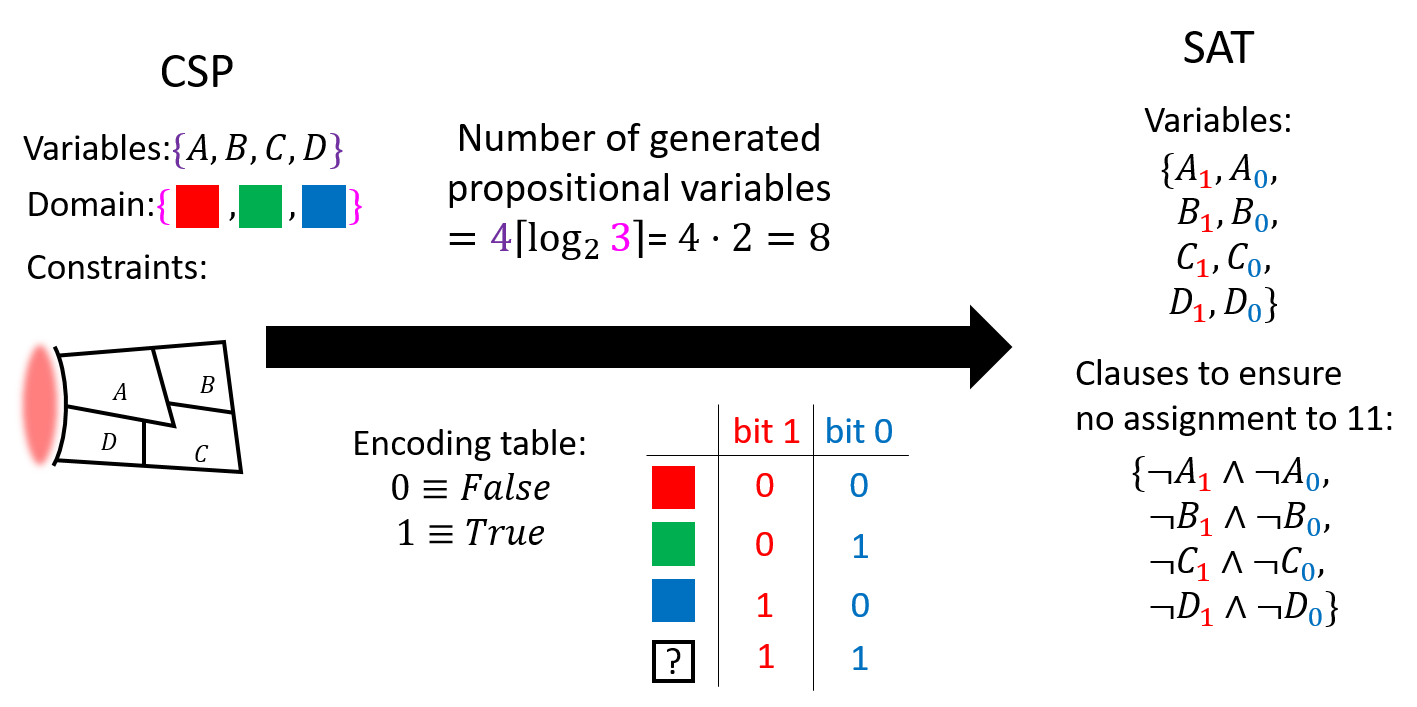
\includegraphics[width=0.85\linewidth]{assets/log_variables}
	\captionsetup{justification=centering,margin=2cm}
	\caption{Encoding CSP variables using log encoding}
	\label{fig:log_variables}
\end{figure}

Notice that the log encoding generates less propositional variables than direct encoding. Anyway, this fact does not improve the performance of DPLL on the generated SAT instance because more steps are required to untangle the problem as discussed later. \ref{subsec:log_proposition}

\subsubsection{Encoding the constraints}
As discussed before, constraints could be unary, binary or n-ary. Since any n-ary constraint can be expanded to multiple binary constraints, the main focus will be on encoding only the unary and the binary constraints.

Encoding unary constraints is straight forward. For example to ensure that a CSP variable $X$ can't be assigned a certain value from its domain encoded in the binary form $01$, we only need to add the following clause to the SAT formula: $\neg (\neg X_1 \wedge X_0) \equiv X_1 \vee \neg X_0$. Remember that the subscript of the propositional variables $X_0, X_1$ corresponds to the position of the bit in the binary form of the CSP value.

Encoding binary constraints can be done in similar manner. For example to encode the CSP constraint $A \neq D$, where $A$ and $D$ can be either green \textcolor{green}{$\blacksquare$} or blue \textcolor{blue}{$\blacksquare$} (i.e. their domain is $\{ \textcolor{green}{\blacksquare}, \textcolor{blue}{\blacksquare} \}$) with the binary representations are \textcolor{green}{$01$} and \textcolor{blue}{$10$} respectively, as show in the figure \ref{fig:binary_constraints_log_encoding}.
\begin{figure}[H]
	\centering
	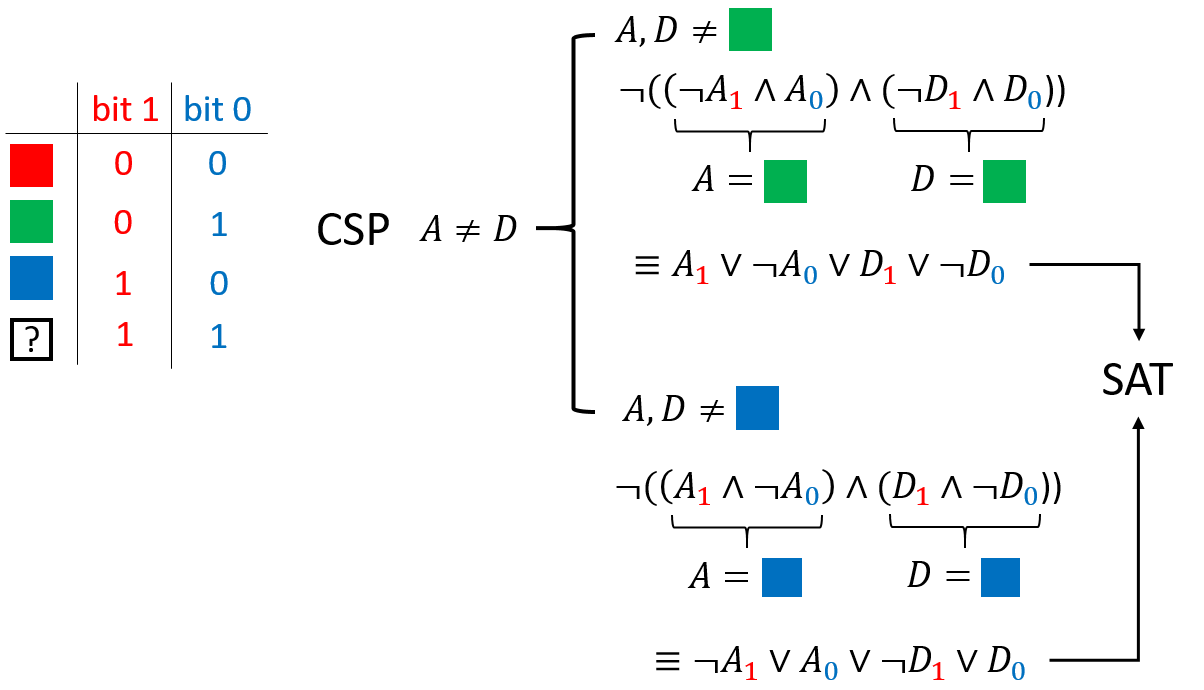
\includegraphics[width=0.7\linewidth]{assets/binary_constraints_log_encoding}
	\captionsetup{justification=centering,margin=2cm}
	\caption{Encoding binary CSP constraint using log encoding}
	\label{fig:binary_constraints_log_encoding}
\end{figure}

\subsubsection{Proposition}\label{subsec:log_proposition}
In spite of the fact that log encoding generate fewer variables on the SAT side than direct encoding, it is easy to see that DPLL applied on log encoded CSP is dominated by FC applied to the original CSP problem assuming equivalent branching heuristics.

\subsubsection{Proof idea}
The proof idea is much the same as direct encoding. We process by comparing the search trees of each algorithm. First we show that both trees must have at least equal number of branches. By Induction on each CSP variable $X$ FC will branch upon it. On the SAT side DPLL will consider all propositional variables corresponding to the same CSP variable ($X_i \dots X_{\lceil \log_2 m \rceil}$), where $m$ is the size of the domain.

Further more, we can exploit the natural logarithmic behavior of log encoding on the search tree to show that DPLL is \textbf{strictly} dominated by FC. This can be done using a simple example. Consider a CSP consists of two variables $A$ and $B$ with domain of size 3 and no constraints. FC will require three branches for each variable to show that this problem is unsatisfiable. Since the size of the domain equals 3, we need at least two bits to represent each CSP variable. Therefore, DPLL must branch at least $2 * 2 * 2 = 8$ times to show that the problem is unsatisfiable (the first 2 represents for the number of variables, the second one for the number of bits, and the last one to indicate branching on each case True or False as discussed before).

\begin{figure}[H]
	\centering
	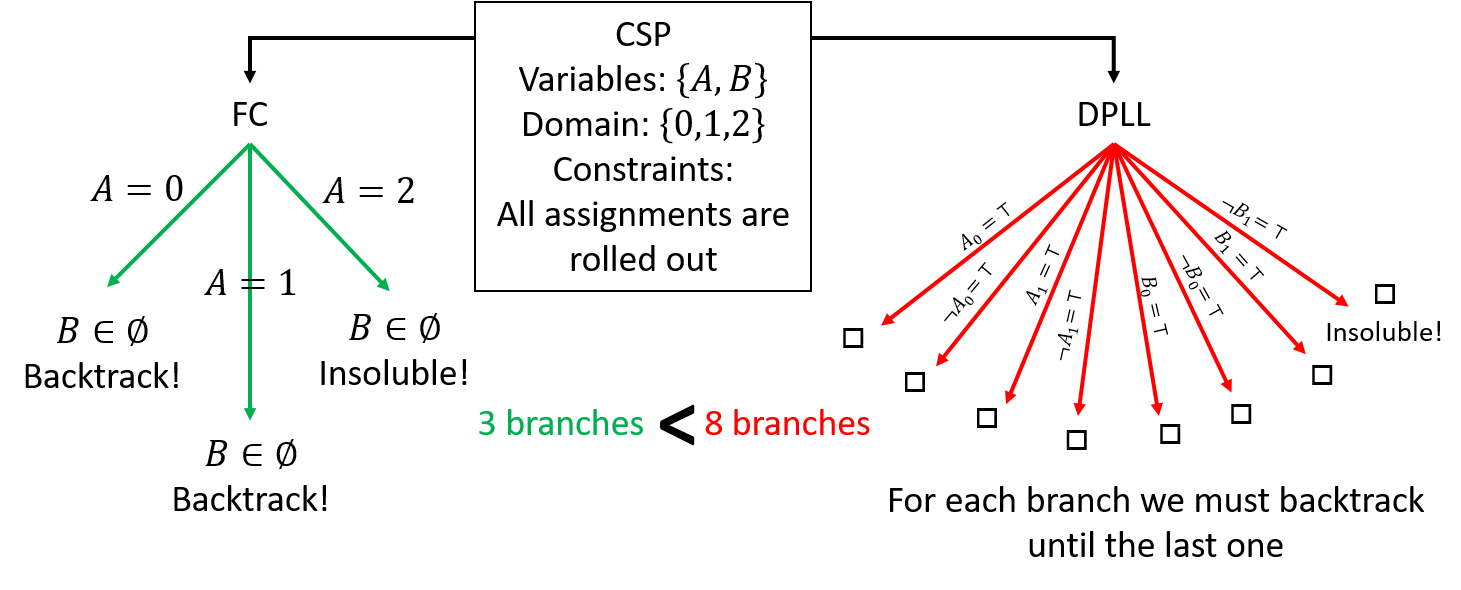
\includegraphics[width=0.85\linewidth]{assets/log_dominated_by_fc}
	\captionsetup{justification=centering,margin=2cm}
	\caption{Seach trees of DPLL and FC for trivial CSP}
	\label{fig:log_dominated_by_fc}
\end{figure}





% !TeX spellcheck = en_US
\subsection{Order encoding}

Order encoding took a different path to approach the problem of transforming CSP into SAT. The essential idea is extending the expressive power of Boolean expressions to represent a whole range of possible values on the CSP side as a comparison.

Despite being simple in its complexity, the order encoding is one if most efficient approaches to encode CSP into SAT and generate a relatively simpler instance that can be solved quickly under the assumption that the right conditions are met.

\subsubsection{Usage}
A lot of the CSP-Solvers are actually based on a SAT-Solver (such as MiniSat). The given CSP is first encoded using order encoding (or a variant of it) and then solved by the SAT-Solver. One of the first prominent award-winning SAT-based constraint solvers called sugar, which is based around the same idea using MiniSat as the underlying SAT-solver \cite{tamura2008sugar}.

\subsubsection{Encoding the variables}
Assuming a consistent CSP domain for the variable $x$ ranging from $l(x)$ to $u(x)$ where $l$ and $u$ represent the lower and upper bounds respectively, a Boolean variable is generated $p_{xi}$ for each value $i$ in the domain of $x$. $p_{xi}$ is semantically equal to $x \leq i$. And therefor $p_{xk}$ for $k = u(x)$ is always True and must be added as its own clause because it must be satisfied.

To facilitate an unambiguous entry point for DPLL, the order encoding adds additional trivial propositional variable  $p_{xj}$ for each CSP  variable $x$ where $j = l(x) - 1$. This variable must be added as its own clause since it's clearly False at all times. Similar variables $p_{xk}$ for  $k = u(x)$ are always True. Both of these clauses $\neg p_{xj} \wedge p_{xk}$ helps the unit propagation rule exploiting the SAT instance of the problem and constraint it by providing boundaries for each variable.

Since $x \leq i$ implies $x \leq i+1$ and $p_{xi}$ means $x \leq i$, we must also encode this fact into our SAT to ensure a consistent assignment of each variable:
$$
x \leq i \rightarrow x \leq i + 1 \quad \equiv \quad
\neg x \leq i \vee x \leq i + 1 \quad \equiv \quad
\neg p_{xi} \vee p_{x(i+1)}
$$

\begin{figure}[H]
	\centering
	
\includegraphics[width=0.7\linewidth]{assets/order_encoding_variables}
	\captionsetup{justification=centering,margin=2cm}
	\caption{An example for encoding CSP variables using order encoding}
	\label{fig:order_encoding_variables}
\end{figure}

\subsubsection{Encoding inequality constraints}
Order encoding works best for the inequality constraints (concretely constraints of the form $\sum_i a_i x_i \leq b$). Other types of constraints will be discussed in the next section \ref{sec:general_constraints}. The efficiency of the order encoding lays in its powerful encoding of entire conflict regions instead of single conflict points (in comparison with log and direct encodings) \cite{tamura2008sugar}. To encode a constraint of the form $\sum_{i=1}^n a_i x_i \leq b$, we must first generate the conflict regions for each variable which is a set of integer tuples $C := \{c_1, \dots, c_n \}$ that satisfies the constraints: 
\begin{align}
	&\sum_{i=1}^n c_i = b - n + 1 \\
	&\bigwedge_{i=1}^n (\min(a_i \cdot x_i) \leq c_i \leq \max(a_i \cdot x_i))
\end{align}

Then the required clauses to encode the constraint are:
\begin{equation}
\forall c_i \in C: \bigvee_{i=1}^n 
\begin{dcases}
	x_i \leq \lfloor \frac{c_i}{a_i} \rfloor \equiv
	 p_{x_i (\lfloor \frac{c_i}{a_i} \rfloor)} &\quad a_i > 0 \\[10pt]
	\neg (x_i \leq \lceil \frac{c_i}{a_i} - 1) \rceil \equiv
	 \neg p_{x_i (\lceil \frac{c_i}{a_i} - 1) \rceil)} &\quad a_i < 0 
\end{dcases}
\end{equation}

\paragraph{Example}
To encode the constraint $x + y \leq 5$ for the unified domain $\{2,3,4\}$ we need to consider the conflict regions $C = \{ (1,3), (2,2), (3,1) \}$, so the following clauses must be included in our SAT formula:
$$
	p_{x1} \vee p_{y3}  \quad(\bullet) \qquad
	p_{x2} \vee p_{y2}  \quad(\times)  \qquad
	p_{x3} \vee p_{y1}  \quad(\circ)
$$

\begin{figure}[H]
	\centering
	\definecolor{cqcqcq}{rgb}{0.7529411764705882,0.7529411764705882,0.7529411764705882}
	\begin{tikzpicture}[line cap=round,line join=round,>=triangle 45,x=1.0cm,y=1.0cm]
	\draw [color=cqcqcq,, xstep=1.0cm,ystep=1.0cm] (0,0) grid (5.5,5.5);
	\draw[->,color=black] (-0.78,0.) -- (5.75,0.);
	\foreach \x in {,1.,2.,3.,4.,5.}
	\draw[shift={(\x,0)},color=black] (0pt,2pt) -- (0pt,-2pt) node[below] {\footnotesize $\x$};
	\draw[->,color=black] (0.,-0.57) -- (0.,5.92);
	\foreach \y in {,1.,2.,3.,4.,5.}
	\draw[shift={(0,\y)},color=black] (2pt,0pt) -- (-2pt,0pt) node[left] {\footnotesize $\y$};
	\draw[color=black] (0pt,-10pt) node[right] {\footnotesize $0$};
	\clip(-0.78,-0.57) rectangle (5.75,5.91);
	\draw [domain=-0.78:5.75] plot(\x,{(--5.-1.*\x)/1.});
	\begin{scriptsize}
	\draw [fill=black] (1.,3.) circle (2.5pt);
	\draw [fill=black] (1.,2.) circle (2.5pt);
	\draw [fill=black] (1.,1.) circle (2.5pt);
	\draw [color=black] (2.,2.)-- ++(-2.5pt,-2.5pt) -- ++(5.0pt,5.0pt) ++(-5.0pt,0) -- ++(5.0pt,-5.0pt);
	\draw [color=black] (2.,1.)-- ++(-2.5pt,-2.5pt) -- ++(5.0pt,5.0pt) ++(-5.0pt,0) -- ++(5.0pt,-5.0pt);
	\draw [color=black] (3.,1.) circle (2.5pt);
	\end{scriptsize}
	\end{tikzpicture}
	\captionsetup{justification=centering,margin=2cm}
	\caption{An example for encoding the constraint $x + y \leq 5$ using order encoding}
	\label{fig:order_encoding_example}
\end{figure}

\subsubsection{Encoding general constraints}\label{sec:general_constraints}
Other types of constraints are replaced by equivalent expressions composed from one or multiple constraints of the form $\sum_i a_i x_i \leq b$ while adding extra conditions (clauses) if necessary.

For example to encode the expression $x < y$ we replace it by $x + 1 \leq y \equiv p_{(x+1)y}$, an equality expression between $x$ and $y$ can be then replaced by $x \leq y \wedge x \geq y \equiv x \leq y \wedge \neg (x < y) \equiv p_{xy} \wedge p_{(x+1)y}$, similarly $x \neq y \equiv x < y \vee x > y$ and so on \cite{tamura2008sugar}.

\subsubsection{Importance}
In theory and assuming worst-time performance, the order encoding is no better than the other type of encodings, but in real-world applications it has been shown that the order encoding have better performance than the direct encoding on instances of the graph coloring and open-shop scheduling problems. \cite{tamura2009compiling}

Moreover, the order encoding, unlike the other encodings discussed earlier, is the first encoding that can translate a CSP into a so called tractable SAT, which means that the SAT problem can be solved by a SAT-solver in polynomial time. However, this statement is true only for certain classes of CSP problems. It has been proven that the following tractable CSP classes can be encoded into a tractable SAT problems using the order encoding: \cite{petke2011order}
\begin{enumerate}
	\item constraint-closed
	\item max-closed
	\item connected row-convex
\end{enumerate}
All the previous classes are some type of formality imposed on the constraints' set of the CSP problem. Comparisons and tables of SAT-solvers performance on the direct, log and order encoding of different tractable CSP instances can be found in \cite{petke2011order}.




% !TeX spellcheck = en_US
\subsection{Hybrid encoding integrating Log and Order encoding}
With the idea of exploiting the pros of each encoding and avoid their cons a new hybrid encoding emerged. Log encoding represents each value in CSP's domain as binary integer and as a result generates small SAT problems regarding the number of propositional variables and the number of constraints (compared to the direct encoding since no additional clauses are required). On the other hand, the order encoding is known for its performance, then it generates additional variables that bounds the SAT problem and make it more liable for being solved directly by the one literal rule using unit propagation instead of branching. But each encoding has its limitations; for instance: the order encoding generate huge SAT instances when the CSP domain or the arity of the constraints becomes large. Likewise, the log encoding suffers from poor performance in general.

\subsubsection{Core idea}
Other encodings have already proposed merging multiple encodings together to benefit from each of them, but no true hybridization have been applied. Each variable was encoded with both types of used encodings and then additional clauses were added to channel both types of generated constraints together. This proposed encoding works without channeling the constraints and using a criterion to determinate the appropriate encoding for each variable. Therefore, the resulted constraints can contain both types of encoded variables and don't require additional constrains channeling. Log and order encodings operates as partial encoding, while their use is controlled by the criterion. The authors proposed the domain product as the classification criterion but other criteria could have been used. \cite{soh2015hybrid}

\subsubsection{Performance test}
The authors implemented their own CSP-Solver and tested it against two sets of benchmark problems. The first set was handmade and the second one was selected from a CSP solver competition. In both tests the hybrid encoding showed better results and superior performance compared to applying the partial encodings alone. Detailed tables with exact figures and details about the test environment are provided in the original paper \cite{soh2015hybrid}. It should be noted that this some problems with high artiy and domain size could be only solved with the hybrid encoding in a reasonable amount of time.

The following Venn diagram in Fig.\ref{fig:hybrid_encoding_venn} shows the number of instances from the second benchmark set solved by each encoding. Clearly the hybrid encoding with 815 solved instances dominates both log and direct encoding. Only 6 problems were unsolvable by the new hybrid encoding, which is the smallest number among the other encodings. The paper \cite{soh2015hybrid} also compares the 3 encodings regarding the average CPU time needed for solving the first benchmark set. As expected, the hybrid encoding correctly inherits the advantages of both encodings and comes out as the clear winner.

\begin{figure}[H]
	\centering

	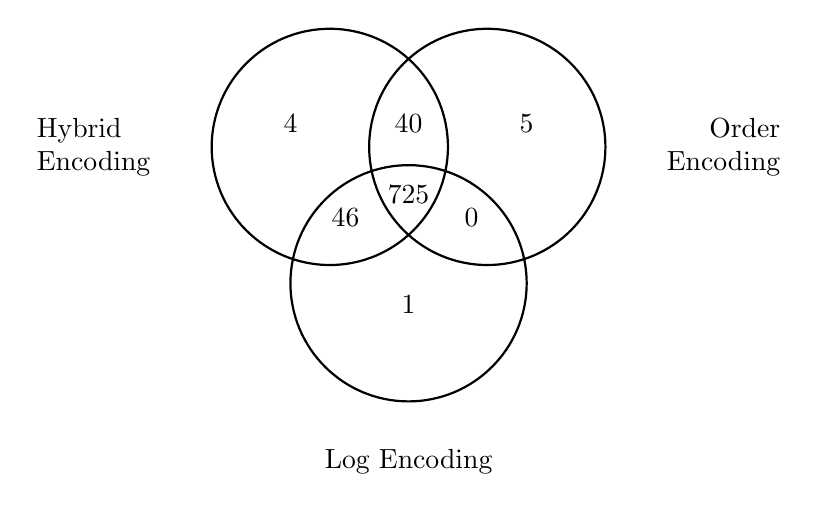
\begin{tikzpicture}[thick]
		 % Draw the circles
		 \draw (0,0) circle (1.5cm);
		 \draw (-60:2cm) circle (1.5cm);
		 \draw (0:2cm) circle (1.5cm);
		 
		 % Label the circles
		 \draw[align=left] (-3,-0) node {Hybrid\\Encoding};
		 \draw (1,-4) node {Log Encoding};
		 \draw[align=right] (5,0) node {Order\\Encoding};
		 \draw (-0.5,0.3) node {4};
		 \draw (1,0.3) node {40};
		 \draw (2.5,0.3) node {5};
		 \draw (0.2,-0.9) node {46};
		 \draw (1,-0.6) node {725};
		 \draw (1.8,-0.9) node {0};
		 \draw (1,-2) node {1};
	\end{tikzpicture}
	
	\captionsetup{justification=centering,margin=2cm}
	\caption{Number of solved instances from the benchmark set by each encoding}
	\label{fig:hybrid_encoding_venn}
\end{figure}

% !TeX spellcheck = en_US
\section{SAT into CSP encodings}\label{sec:sat_to_csp}
In this section, we discuss the opposite direction by introducing several ways for encoding SAT into CSP and briefly summarize the pros and cons of each encoding.

\subsection{Dual encoding}
For each clause in the CNF-formatted SAT a CSP variable is generated. The domain of each variable consists of the possible truth assignments that satisfies the corresponding clause expressed as a tuple. Any two clauses sharing the same propositional variable must also have a binary constraint between their respective dual variables. These constraints assure consistent assignment of the common propositional variable such that no variable is assigned two different values at the same time. 

The following example shows how we could encode a SAT problem with two clauses and one common propositional variable. Considering the clauses: $x_1 \vee x_2$ and $x_3 \vee \neg x_2$. The first clause results in the dual variable $D_1$ with the domain $\{(T,T),(T,F),(F,T)\}$ where $T$ and $F$ represent the truth value of the corresponding Boolean variable at the respective position within the tuple. The second clause results in $D_2 \in \{(T,F),(T,T),(F,F)\}$. Since $x_2$ appears in both clauses, we must ensure that it will not have different values in each variable through the binary constraint: $D_1[2] = \neg D_2[2]$ which assures that the second element of the tuple assigned to $D_1$ is the inverse of the second element of the $D_2$ tuple.

\subsubsection{Theoretical comparison}
It has been proven \cite{walsh2000sat} that FC on the dual encoded SAT instance does more work than DPLL on the original problem. The proof is based on the fact that a truth assignment under unit propagation in DPLL implies an elimination of contradictory values on the CSP side. By induction, we can see that generating the empty clause in DPLL (which indicates that the problem is unsatisfiable regarding the current branch) implies a domain wipe out after applying arc-consistency by FC.

\subsection{Hidden variable encoding}
Just like dual encoding, the hidden variable encdoing assign a dual variable for each SAT clause. Furthermore, each propositional variable $x_i$ is simulated on the CSP side with a binary variable $X_i \in \{T,F\}$. This encodings allows constraints to be easily formulated in terms of thier binary variables. For example the clause $x_1 \vee \neg x_2$ results in one dual variable $D_1 \in \{(T,F),(F,F),(T,T)\}$ and two binary CSP variables $X_1, X_2$ and additionally the coupling constraints $D_1[1] = x_1$ and $D_1[2] = \neg x_2$ which constraints any assignment of the elements of the tuple assigned to $D_1$ to be consistent with the propositional variables $x_1,x_2$ represented by their CSP counterparts $X_1,X_2$.

\subsubsection{Theoretical comparison}
The hidden variable encoding maintain equivalent relation between assigning truth values committed by one literal rule on the DPLL side and eliminating contradictory values by enforcing arc-consistency by FC/MAC on the node level. This translates to equivalence relation between generating empty clauses and empty domain \cite{walsh2000sat}. This in turn means that DPLL will essentially branch in general as much as FC/MAC applied to the encoded version of the same problem, and the same amount of work is expected by each algorithm.

\subsection{Literal encoding}
The literal encoding express each clause as a variable with a domain consisting of propositional variables' values that satisfy the corresponding clause. Constraints are required between any CSP variables if and only if their domains contain contradictory propositional variables. For example the clauses $x_1 \vee x_2$ and $x_3 \vee \neg x_2$ can be expressed as the following variables $D_1 \in \{x_1, x_2\}, D_2 \in \{x_3, \neg x_2\}$ and the constraint $\neg (D_1 = x_2 \wedge D_2 = \neg x_2)$ which rules out this inconsistent assignment for $x_2$.

\subsubsection{Theoretical comparison}
This encoding shows similar results as the hidden variable encoding regarding the relation between generating the empty clause and empty domains as a result of enforcing arc-consistency. Anyway MAC is strictly dominated by DPLL applied to the original. Strictness can be proved easily by contradiction. Consider any unsatisfiable $k-$SAT instance (i.e. a SAT problem with $k$ propositional variable) with $2^k$ clauses where $k > 2$. DPLL needs $2^{k-1}$ branch to arrive at the empty clause while MAC takes $k!$ branches regardless of the used heuristics \cite{walsh2000sat}.

\subsubsection{Advantage of literal encoding}
CSP domain size can have great impact on the performance of any arc-consistency based algorithm (like MAC or FC) and must be taken into consideration. Let $n$ be the number of SAT clauses. Dual and hidden variable encodings generate CSP instance with domain size in the order of $\mathcal{O}(2^n)$ while the literal encoding generate CSP instances with domain size of $\mathcal{O}(n)$
 

\section{Conclusion}\label{sec:conclusion}
We discussed some mappings between the constraint satisfaction problem (CSP) and the Boolean satisfiability problem (SAT). Some theoretical background has been introduced and based on general comparing criterion the encodings have been analyzed and compared against each other. It has been shown that the choice of an encoding has a large impact on the efficiency and solvability of the generated problem. Encoding CSP into simpler SAT problem has led to efficient instances of the original problem that can be solved quickly. This claim was supported with theoretical arguments and proofs specially in the case of some tractable CSP classes encoded using the order encoding. Based on similar encoding techniques various new SAT-based constraint solves have been developed. On the other hand, a variety of SAT to CSP encodings have been introduced. Although no SAT to CSP encoding has proven itself to be superior, a clearer picture of the relation between CSP and SAT has emerged and further studies can build upon these results.

%%% Bibliography
\newpage
\nocite{*}
\bibliographystyle{ieeetran}
\bibliography{bibliography}

\end{document}